\section{SMC model} \label{sec:smc_model}
\Gls{smc} is chosen because \gls{cora} handles randomness poorly making it inadequate to perform robustness check, because of its deterministic approach, compared to \gls{smc} which can perform undeterministic choices. This section will focus on how a \gls{smc} model can be constructed to provide further insight about the schedules robustness produced by the \gls{cora} model. Additionally the \gls{smc} model will need variables mentioned in \myref{sec:read_input}.

Since \gls{smc} allows clocks to have non-linear rate along with rational numbers, it is possible to implement \gls{kibam}, see \myref{sec:kibam}. The advantage of using the battery model over ideal, implemented in \gls{cora}, is that \gls{kibam} is pessimistic in the sense that \gls{kibam} tends to underestimate the actual battery levels. Because of this \gls{kibam} will be implemented in the \gls{smc} model, instead of the ideal

Our \gls{smc} model consist of four templates plus one instance of a template for each window described in the payload specification. However, it is required that at least one window is defined in the input. This makes a total of 5 plus templates, which are Processor, Insolation, EnergySource, Scheduler, and PayloadWindow(i).\\ 
The \gls{smc} model is based on a UPPAAL implementation of \gls{kibam} \cite{battery_aware_scheduling}, and our \gls{cora} model. The UPPAAL implementation of \gls{kibam} covers scheduling with uncertainty, combined with capturing battery levels during execution of the schedule. \\
The rest of this section we will go over each of the important points in the model, this include the concept of recharging, windows for payloads, payload dependencies ect. 
\ofx{det er ikke blevet beskrevet hvorfor vi laver denne model! ud fra dette ville jeg gætte på det er for KiBaM}

\subsection{Processor}
The initial version of this template was based on a the UPPAAL implementation of \gls{kibam}, which we have then modified to fit our context. The processor template describes the status of the nanosatellites processor, it indicates if it is currently executing a payload, waiting for a payloads deadline to be reached or idling.\\
As the \gls{smc} model receives a schedule from \gls{cora} it does not need to find a payload to execute, instead it will look for the next entry in the array describing what payloads to execute, such an array can be seen in \cref{lst:queue}. This template is responsible for updating the queue, and keeping track of how many payloads have been skipped, and the earnings, in regards to the specified profit.\\
The processor in this model also differs form the one in the \gls{cora} model in the way that in this model, the processor may remain in \uppLoc{Running} for a varying amount of time instead of just the worst execution time for the payload.\\
It synchronises with the scheduler template onthe channel \uppSync{ready!} and then awaits a synchronisation on either \uppSync{run?} or \uppSync{skip?}, while the scheduler determines what to do with the next payload.
\begin{figure}[H]
	\begin{lstlisting}[language=my_c, caption={Payload queue with start times, extracted from the \gls{cora} model}, label=lst:queue, firstnumber=53]
	.
	.
	.
//from cora
int Queue[NumberOfPayloads] = {4, 0, 1, 0, 1, 0, 1, 0, 2, 0, 2, 0, 3, 0, 3, 0};
const int RunStart[NumberOfPayloads] = {0, 50, 100, 140, 190, 230, 280, 320, 370, 410, 460, 500, 550, 590, 640, 680};
	\end{lstlisting}
\end{figure}




\begin{figure}[H]
	\centering
	\begin{tikzpicture}
	%Locations
	\node [init] (l0) [label={[align=left]above:\textcolor{name}{Init}}] {$\cup$};
	\node [location] (l1) [right of=l0, xshift=40mm, label={
		[align=left]above:
		\textcolor{name}{Idle}},
	label={
		[align=center]below:
		\textcolor{invariant}{totalTime <= RunStart[payloadNumber]}
	}] {};
	\node [location] (l2) [right of=l1, xshift=80mm, label={
		[align=left]above:
		\textcolor{name}{Ready}
	}] {};
	\node [location] (l3) [below of=l0, yshift=-40mm, label={
		[align=left]below:
		\textcolor{name}{Done}
	}] {};
	\node [location] (l4) [below of=l1, yshift=-40mm, label={
		[align=left]below:
		\textcolor{name}{Wait}\\
		\textcolor{invariant}{x <= D}
	}] {};
	\node [location] (l5) [below of=l2, yshift=-40mm, label={
		[align=left]below:
		\textcolor{name}{Running}\\
		\textcolor{invariant}{x <= W}
	}] {};
	\path[->,black, thick] (l0) edge node [midway, above][align=left]{
		\textcolor{update}{t=0,i = IIdle,}\\
		\textcolor{update}{setActive()}} (l1);
	\path[->,black, thick] (l1) edge node [midway, above][align=center]{
		\textcolor{guard}{totalTime >=RunStart[payloadNumber]}\\
		\textcolor{sync}{ready!}\\
		\textcolor{update}{x=0, t=0,}\\
		\textcolor{update}{deadline()}} (l2);
	\path[->,black, thick] (l2) edge node [midway, right][align=left]{
		\textcolor{sync}{run?}\\
		\textcolor{update}{x := 0,}\\
		\textcolor{update}{setActive(),}\\
		\textcolor{update}{enqueue()}\\
		\textcolor{update}{earnings +=}\\
		\textcolor{update}{Profit[active]}} (l5);
	\path[->,black, thick] (l2) edge node [midway, left][align=left]{
		\textcolor{sync}{skip?}\\
		\textcolor{update}{payloadNumber ++,}\\
		\textcolor{update}{skipped()}} (l4);
	\path[->,black, thick] (l5) edge node [midway, below][align=left]{
		\textcolor{guard}{x >= B}\\
		\textcolor{update}{dequeue(), active = -1,}\\
		\textcolor{update}{payloadNumber ++}} (l4);
	\path[->,black, thick] (l4) edge node [midway, left][align=left]{
		\textcolor{guard}{x >= D \&\&}\\
		\textcolor{guard}{!done()}\\
		\textcolor{update}{setActive()}} (l1);
	\path[->,black, thick] (l4) edge node [midway, below][align=left]{
		\textcolor{guard}{done()}\\
		\textcolor{update}{on = false,}\\
		\textcolor{update}{active = -1}} (l3);
	\end{tikzpicture}
	\caption{Processor template}
	\label{fig:smc_P}
\end{figure}

\subsection{Scheduler}
When the location \uppLoc{Ready} from Processor is active, two transitions is available to either execute or skip the current payload, each of the transitions are dependent on the scheduler template seen in \cref{fig:smc_S}. This template is responsible for determining if a payload can be run based on all of the restrictions defined, in the payload and environment description, by the user. This includes dependencies, windows, and the battery levels. It checks the windows, dependencies, and the maximum amount of runs per reset, whereas for the battery level it calculates an estimate of what it would be after executing the payload, this is done for both the available, bound and total level.
This is necessary to ensure that a payload does not draw more power than currently available. All of these checks are done on the transition that broadcast \uppSync{run!} indicating that it is safe to execute the payload. \\
If for some reason it is not possible to perform the transition it waits until we either have recharged enough energy or a chance in the windows have occurred, allowing for execution of the payload. If we are not able to perform the payload before the deadline, which is calculated by subtracting worst from the payload deadline, then the other transition is activated leading to a skip of the payload. With dependencies this can have significant consequences to the schedule because the next payload in the schedule may have depended the skipped payload thus resulting in a chain of skipped payloads.

\begin{figure}[H]
	\centering
	\begin{tikzpicture}
	%Locations
	\node [init] (l0) {};
	\node [location] (l1) [right of=l0, xshift=40mm, label={
		[align=left]right:
		\textcolor{invariant}{t <= Payloads[Queue[payloadNumber]][2] - }\\
		\textcolor{invariant}{Payloads[Queue[payloadNumber]][1]}
	}] {};
	\path[->,black, thick] (l1) edge[bend left=50] node [midway, below][align=left]{
		\textcolor{guard}{t == Payloads[Queue[payloadNumber]][2] - }\\
		\textcolor{guard}{Payloads[Queue[payloadNumber]][1]}\\
		\textcolor{sync}{skip!}
	} (l0);
	\path[->,black,thick] (l0) edge node [midway, below][align=left]{
		\textcolor{sync}{ready?}} (l1);
	\path[->,black,thick] (l1) edge[bend right=45] node [midway, above][align=left]{
		\textcolor{guard}{on \&\& mayRun() \&\&}\\
		\textcolor{guard}{0.1 < a * exp(-k2*W)+}\\
		\textcolor{guard}{(((a+b)*k2*c-(Costs[active]+IIdle))*(1.0-exp(-k2*W))}\\
		\textcolor{guard}{-(Costs[active]+IIdle)*c*(k2*W-1.0+exp(-k2*W)))/k2}\\
		\textcolor{guard}{\&\& Threshold < checkB(a,b,totalTime)}\\
		\textcolor{sync}{run!}\\
		\textcolor{update}{runs[active] ++,}\\
		\textcolor{update}{totalRuns[active] ++}
	} (l0);
	\end{tikzpicture}
	\caption{Scheduler template}
	\label{fig:smc_S}
\end{figure}

\subsection{Payload Window}
The PayloadWindow template can be found in \cref{fig:smc_OW}, with three locations that each have an in and out going transition creating a loop between them. The overall functionality is similar to the template PayloadWindow in the \gls{cora} model. Like in the \gls{cora} model, one instance of PayloadWindow occurs for each defined window. However, in this model it is independent from the rest of the model, in the sense that there are no synchronisations, and is only responsible for keeping track of the window by updating a global variable when a change occur.
%When the first transition, from the initial location, is taken it indicates that the window is now active by changing the global variable \uppVar{inWindow[id]} to 1. When time has passed and window is no longer inside the window the next transition is taken, changing \uppVar{inWindow[id]} to 0. lastly when a full orbit has been performed it resets the clock \uppVar{wtime} with the last transition ending in the initial location.


\subsection{Energy Source} \label{subsec:energy_src}

During the entire schedule we need to keep track of the battery level, as previously mentioned this is done using \gls{kibam}. It is needed to calculate the values of \uppVar{a} and \uppVar{b}, and enable the battery model to recharge\cite{battery_aware_scheduling}. To add the capability of recharging a new location is added to ensure that \uppVar{b} can not exceed its maximum capacity, which is calculated based on the total capacity, so when the model enter the new location it will not add the values of recharge to \uppVar{b}. Additionally a guard is set on the transition leading back to \uppLoc{Charging}, that says \uppVar{b} needs to drain a small amount of power, before going back to the initial location. This is done to prevent damaging the battery further. The final template can be found in \cref{fig:smc_ES}.

In \myref{sec:kibam} we described how \gls{kibam} worked as a function of time that calculate the available and bound wells at time t, but given we store these and calculate the change to them each time tick, a more elegant implementation can be constructed\cite{battery_aware_scheduling}. 
In the model \uppVar{a} and \uppVar{b} are represented by clocks and each passing tick updates the cost on clock \uppVar{a} and \uppVar{b}. This mean that we only need to find the actual increase and decrease to them. This is done using the invariants seen in \cref{eq:calcA} and \cref{eq:calcB}\cite{battery_aware_scheduling}.
\begin{equation}\label{eq:calcA}
	\uppInv{a' == -i+k*(b/(1-c)-a/c)} 
\end{equation}
\begin{equation}\label{eq:calcB}
	\uppInv{b' == -k*(b/(1-c)-a/c)+(insolation * RechargeRate)}
\end{equation}

In \cref{eq:calcA} and \cref{eq:calcB} we see the constant $k$, \uppVar{k} determines the flow rate from \uppVar{b} to \uppVar{a}, to check the imbalance between the the two we divide with the ratio of the wells. Also we see the variable $i$, \uppVar{i} is the current which is always drawn from the battery, this is a combination of \uppVar{IIdle} and \uppVar{Costs[active]} depending on the status of the processor. If a payload is currently being executed $i$ is as seen in \cref{eq:calcI}.

\begin{align}\label{eq:calcI}
\begin{split}
	If Processor.Running & \; \uppVar{i} = \uppVar{IIdle} + \uppVar{Costs[active]} \\
	Otherwise	& \; \uppVar{i} = \uppVar{IIdle}
\end{split}
\end{align}


So for example if the battery has a capacity of $3000$ and a ratio $c = 0.2$ this means that the bound capacity will be $2400$ and the available will be $600$. If we were to calculate the imbalance like so $(b/(1-c)-a/c)$, this would result in zero because $b/(1-c)$ would be $3000$ and $a/c$ would be $3000$. Consider a payload had just taken $100$ from available in a single tick, the equation would now be $(2400/(1-0.2)-500/0.2)$ resulting in $500$ this would then be multiplied by k to give us the rate of how much from bound would be needed to add to available. The same is done for the bound capacity but instead of multiplying by k we multiply by minus k resulting in the value that should be subtracted from the bound well.

In \cref{eq:calcB} we also see the product of \uppVar{insolation} and \uppVar{RechargeRate} being added to \uppVar{b}, when we are in eclipse from the sun, \uppVar{insolation} is false resulting in no recharge being added to \uppVar{b}.

With these changes to the \gls{smc} model we are able to run a schedule with payloads, that have windows and dependencies, with the capability of recharging the battery based on insolation, now we only need to consider what queries should be run in order to give the most usable data for the users.


%Where the \gls{cora} model finds a trace, the \gls{smc} model will try and rerun the produced trace. This means the \gls{smc} model will execute tasks in the exact same order as the \gls{cora} model.% As this model implements KiBaM it gives a fairly accurate representation of the energy consumption. 

%\Cref{fig:cost_schedule} and \cref{fig:solar_task}, shows the different templates used in the \gls{smc} model. To the left of \cref{fig:cost_schedule} are the energy source. The energy source is responsible for updating the remaining available and bound energy, and in case there are no more available energy, it will synchronise with the scheduler which will then stop running more tasks.
%On the right of \cref{fig:cost_schedule} is the scheduler, it awaits a synchronisation from the tasks in order to ensure that they are ready for execution. The scheduler then estimates if running another task will deplete the battery. If this is the case it will transition back to the initial location preparing to run another task. If running another task would not deplete the battery, the task will be run.

%\begin{figure}[H]%
%	\centering
%	\subfloat
%	{{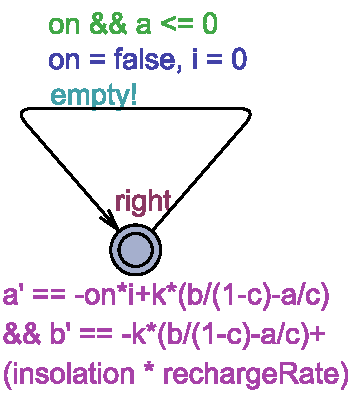
\includegraphics[width=4cm]{graphics/smc_costhandler.pdf} }}%
%	\qquad
%	\subfloat
%	{{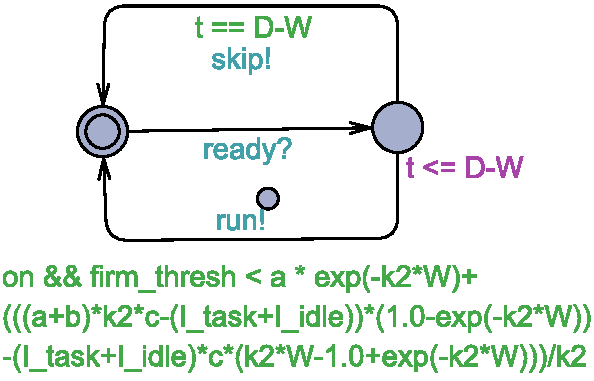
\includegraphics[width=6cm]{graphics/smc_scheduler.pdf} }}%
%	\caption{The \gls{smc} model's energy source(left) and scheduler(right)}%
%	\label{fig:cost_schedule}%
%\end{figure}

%On the left side of \cref{fig:solar_task}, we see the template for the orbit time. It is here assumed that the satellite will spend half its orbit in insolation where it is possible to recharge the battery. It switches the variable \uppVar{Insolation} between true and false, which is used in the calculation of the bound energy.\afx{Kom tilbage hertil når at kibam afsnittet er frdigt. Uddyb om hvordan vores mplementation reflektere teorien fra \cref{sec:kibam}}\\
%The right side of \cref{fig:solar_task} is the template for a task, this indicates that a task can be, ready to be run, running, and inactive. When a task is not running the consumption is lower as indicated by \uppVar{i = I\_idle} which represents the background load of other minor tasks that are not modelled.

%\begin{figure}[H]%
%	\centering
%	\subfloat
%	{{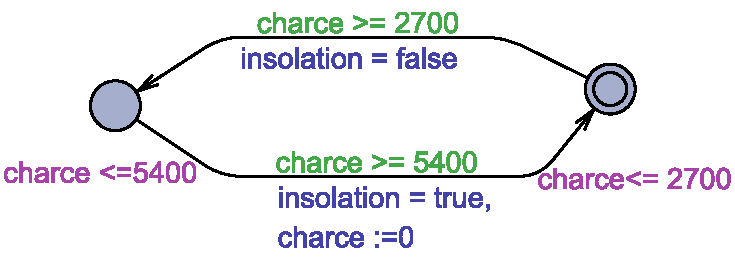
\includegraphics[width=8cm]{graphics/smc_solar.pdf} }}%
%	\qquad
%	\subfloat
%	{{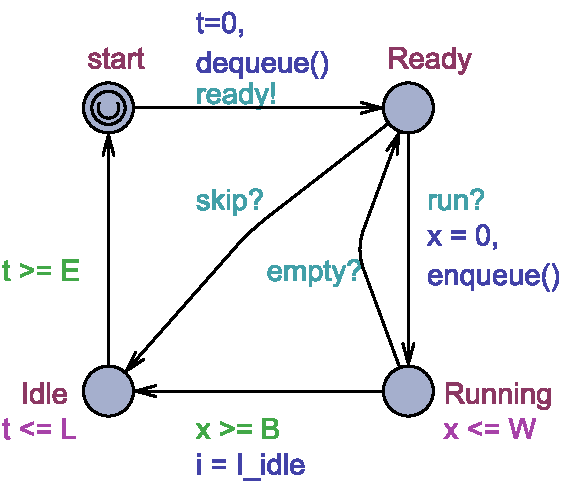
\includegraphics[width=6cm]{graphics/smc_task.pdf} }}%
%	\caption{The \gls{smc} model's representation of solar panels(left) and a task(right)}%
%	\label{fig:solar_task}%
%\end{figure}
%Since the model is made in UPPAAL \gls{smc} we are able to run statistical queries asking for the chance of the available energy falling below some threshold, or to simply track the value of the bound and available energy over time for some specified amount of runs. Examples of such queries can be seen in \cref{eq:pr_low_a_sim_ab}, which indicates, first the chance that the battery level will fall below $55\, \%$ within $43200$ time units. Assuming the time unit is in seconds the example query is for 12 hours. The other query is a simulation of the avilable and bound energy over the same amount of time.\\
%\begin{align}
%Pr[<= 43200] \quad(a <= (c/100)*55)		\nonumber \\
%simulate \quad 1 \quad [<=432000] \quad \{a,b\} 
%\label{eq:pr_low_a_sim_ab}
%\end{align}

%The advantages of running these queries is, that even though the runs in \gls{cora} conclude that a schedule is viable, the probability query may be able to find that running the trace could lead to energy depletion. Also tacking the state of the battery may help to see the effect of the solar panels and the tasks stress on the battery. This is relevant as one or two repetitions of the schedule may not deplete the battery but perhaps ten would, in such case it may be relevant to change some parameters and run it again.